%% LaTeX Beamer presentation template (requires beamer package)
%% see http://bitbucket.org/rivanvx/beamer/wiki/Home
%% idea contributed by H. Turgut Uyar
%% template based on a template by Till Tantau
%% this template is still evolving - it might differ in future releases!

%% Template edited by Panagiotis Adamopoulos {padamopo}@stern.nyu.edu

\documentclass{beamer}
 
\mode<presentation>
{
\usetheme{NYU}

\setbeamercovered{transparent}
}

\usepackage[english]{babel}
\usepackage[latin1]{inputenc}

% font definitions, try \usepackage{ae} instead of the following
% three lines if you don't like this look
\usepackage{mathptmx}
\usepackage[scaled=.90]{helvet}
\usepackage{courier}

\usepackage{float}
\usepackage{wrapfig}


\usepackage[T1]{fontenc}

\usepackage{comment}
%usepackage{appendixnumberbeamer}
%\usepackage{amsmath}
\usepackage{pgfpages}
% citations


\usepackage{caption}
\usepackage{subcaption}
\usepackage[font={scriptsize}]{caption}
\captionsetup[figure]{labelformat=empty}
\captionsetup[subfigure]{labelformat=empty, font=scriptsize, justification=centering}
\usepackage[export]{adjustbox}

\usepackage[square,numbers]{natbib}
\bibliographystyle{abbrvnat}
\renewcommand{\bibsection}{\subsubsection*{\bibname } }

%\usepackage{natbib}
%\bibliographystyle{unsrtnat}
%\bibpunct{(}{)}{;}{a}{,}{,}
%\def\citeapos#1{\citeauthor{#1}'s (\citeyear{#1})}
%\renewcommand{\bibsection}{\subsubsection*{\bibname } }

\graphicspath{ {images/} }
\title{Quality Assurance In Microservice Architectures}

%\subtitle{}

% - Use the \inst{?} command only if the authors have different
%   affiliation.
%\author{F.~Author\inst{1} \and S.~Another\inst{2}}
\author{Krishnan Chandran \and Irina Barykina} 

% - Use the \inst command only if there are several affiliations.
% - Keep it simple, no one is interested in your street address.
\institute[NYU]
{
Department of Informatics,\\
Intelligent Adaptive Systems, UHH\\
}

\date{2016}


% This is only inserted into the PDF information catalog. Can be left
% out.
\subject{Subject}



% If you have a file called "university-logo-filename.xxx", where xxx
% is a graphic format that can be processed by latex or pdflatex,
% resp., then you can add a logo as follows:

% \pgfdeclareimage[height=0.5cm]{university-logo}{university-logo-filename}
% \logo{\pgfuseimage{university-logo}}



% Delete this, if you do not want the table of contents to pop up at
% the beginning of each subsection:
%\AtBeginSubsection[]
%{
%\begin{frame}<beamer>
%\frametitle{Outline}
%\tableofcontents[currentsection,currentsubsection]
%\end{frame}
%}

% If you wish to uncover everything in a step-wise fashion, uncomment
% the following command:

%\beamerdefaultoverlayspecification{<+->}

\begin{document}

\begin{frame}
\titlepage
\end{frame}

%\begin{frame}
%\frametitle{Outline}
%\tableofcontents
% You might wish to add the option [pausesections]
%\end{frame}

%==============================
% Theory section
%==============================
\section{Outline}
\begin{frame}
	\frametitle{Outline}	
	\framesubtitle{}
	\begin{itemize}
		\item What is Quality Assurance?
 		\item QA is easy, isn't it?
		\item QA on Development stage.
		\item QA on Deployment stage.
		\item QA after Release.
		\item Conclusion.
	\end{itemize}
\end{frame}

%===============================
% Introduction
%===============================
\section{Introduction}
\begin{frame}
	\frametitle{Introduction}	
	\framesubtitle{}

\begin{definition}
Quality Assurance refers to planned and systematic production processes that provide confidence in a product's suitability for its intended purposes.
\end{definition}
	\begin{itemize}
 		\item QA must prevent bugs and failures, not identify them.
		\item QA is wasteful on the last stages of development cycle.
	\end{itemize}
\end{frame}

%===============================
% Challenges
%===============================
\section{Challenges}
\begin{frame}
	\frametitle{Introduction}	
	\framesubtitle{Challenges}


	\begin{itemize}
		\item unpredictable timely availability for testing
		\item hard to perform exhaustive integration testing
		\item separated logs and data storages
		\item hard to maintain proper configuration of testing environments
		\item \textbf{\textit{but (!)}} easy to organize low-level testing and catch most of the bugs early
	\end{itemize}
\end{frame}


%===============================
% Example
%===============================
\section{Case study}
\begin{frame}
	\frametitle{Introduction}	
	\framesubtitle{Case Study}
	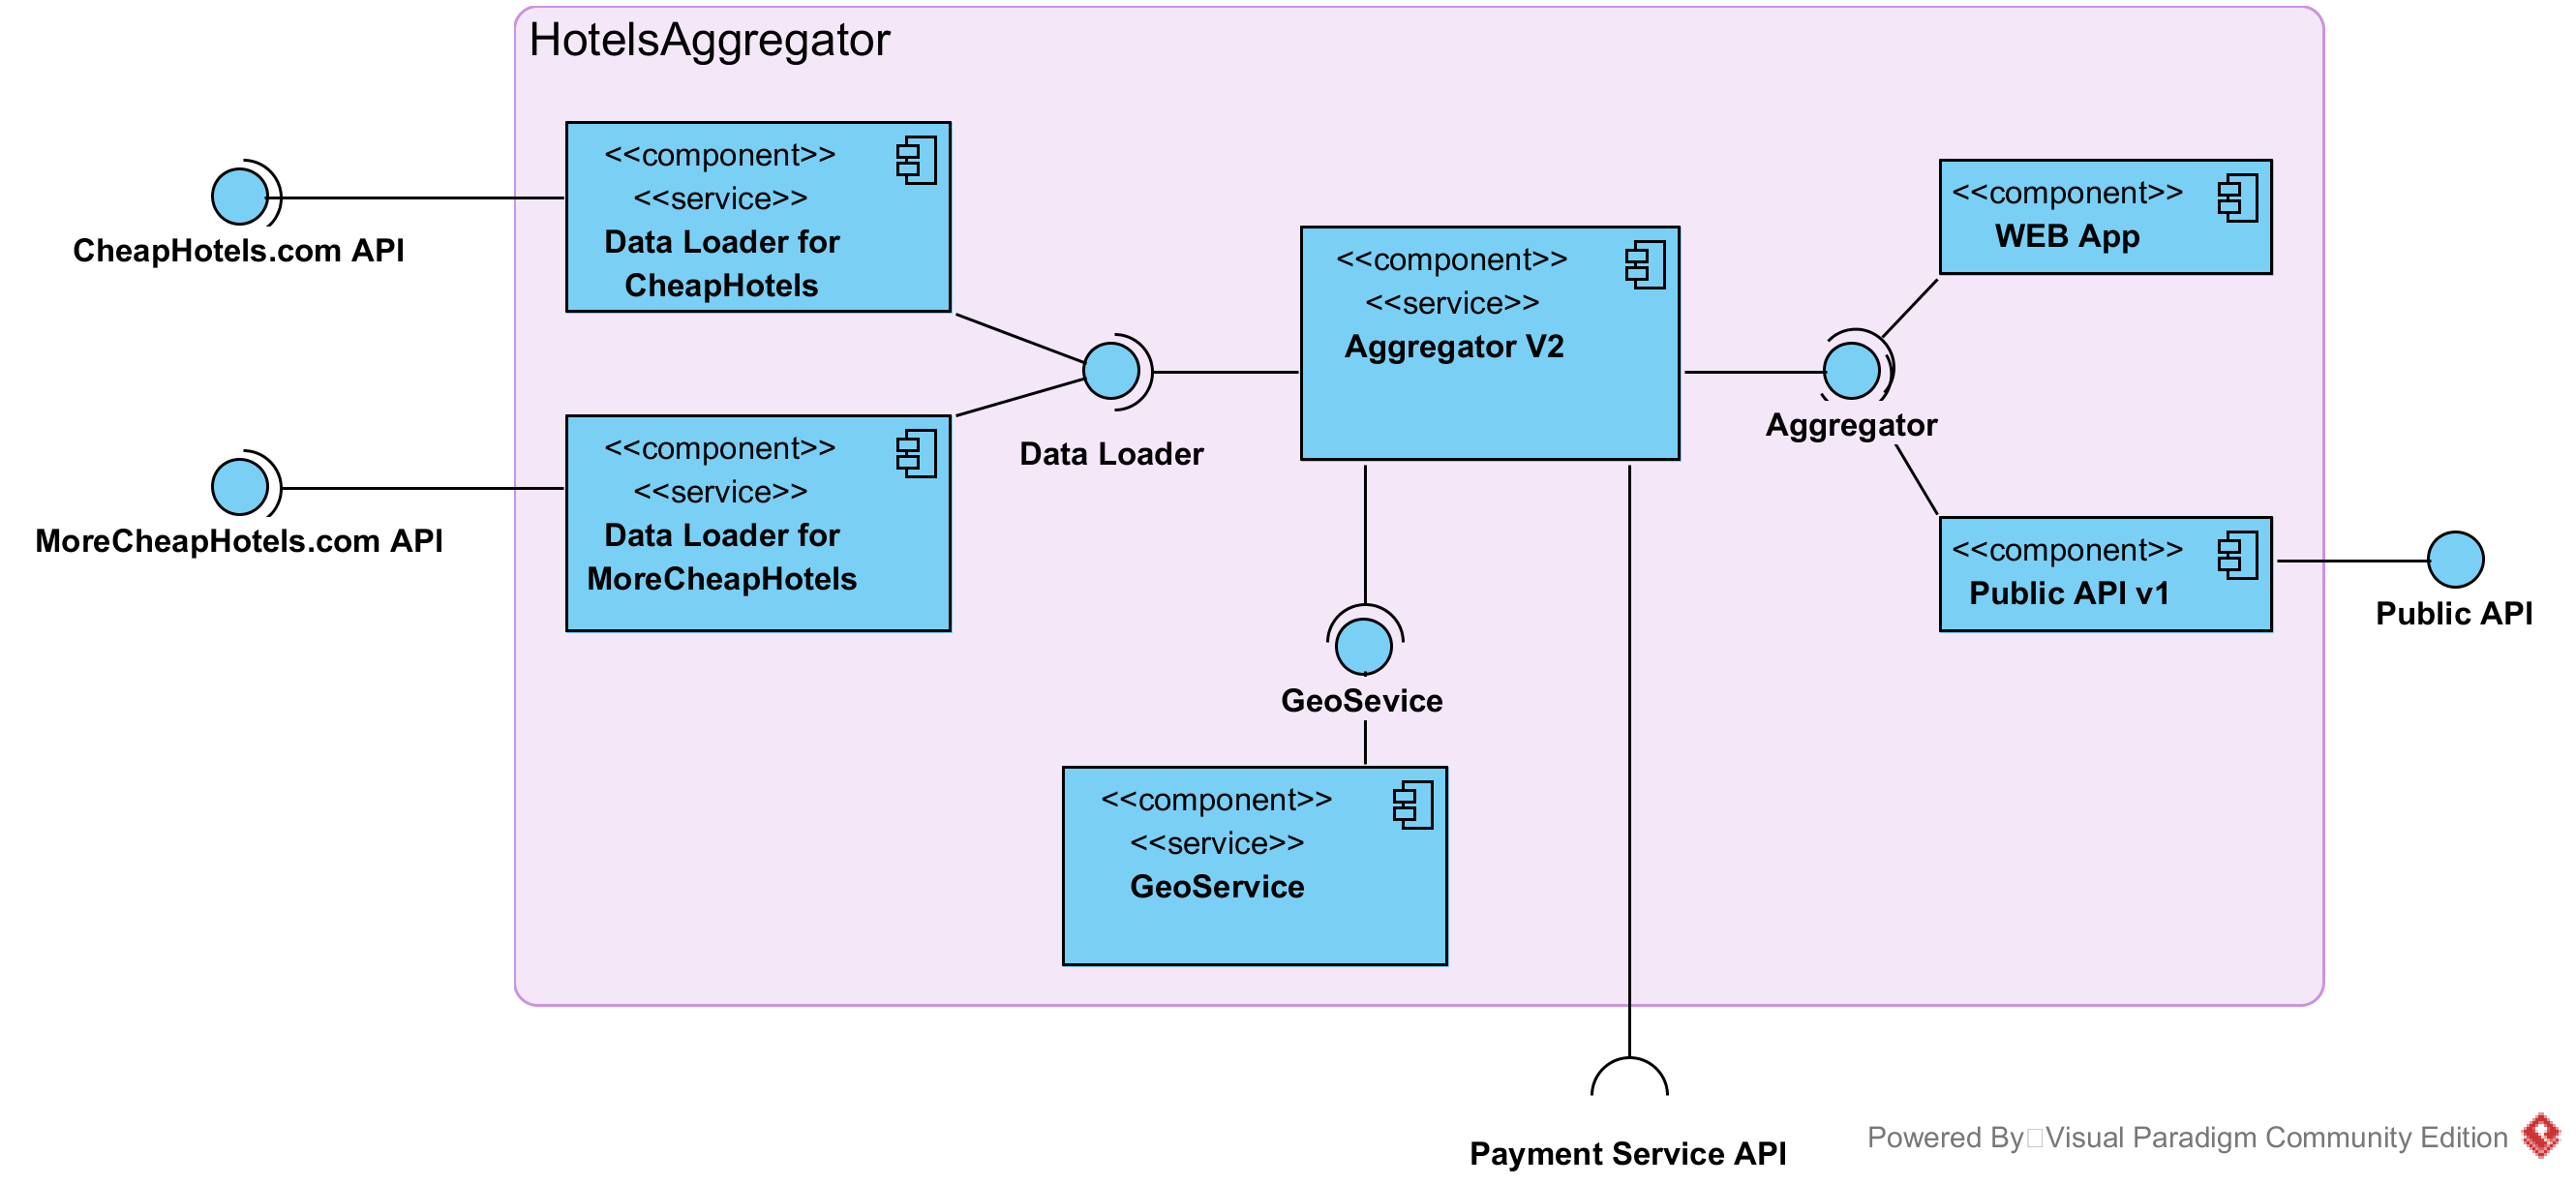
\includegraphics[ scale=0.5]{example}
\end{frame}


%===============================
% Test Pyramid
%===============================
\section{Testing Strategies}
\begin{frame}
	\frametitle{Test Pyramid}	
	\framesubtitle{A balanced test portfolio }
Mike Cohen's Test Pyramid

	\begin{figure}
		\begin{center}
 			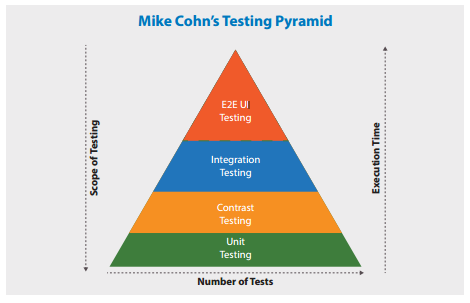
\includegraphics[ scale=0.8]{TestPyramid}
 					\end{center} % image is from Infosys White Paper - Add Reference 
	\end{figure}

\end{frame}

%===============================
% Unit Test - To be revised
%===============================


\begin{frame}
	\frametitle{Types of Tests}	
	\framesubtitle{Applying the layers in a microservice }
Unit Tests
\begin{columns}
 \begin{column}{.49\textwidth}
	\begin{itemize}
		\uncover<1->{\item Coverage limited to individual components}
		\uncover<1->{\item Useful in services, resources, repositories, and adapters }
		\uncover<1->{\item "every build should run the tests, and a failed test should fail the build"}
		\uncover<2->{\item "Solitary Unit Test and Sociable Unit Test"}	
		\uncover<2->{\item "Also a relevant design tool when combined with TDD"}
	\end{itemize}
\end{column}
\begin{column}{.49\textwidth}
	\begin{figure}
		\begin{center}
 			\only<1>{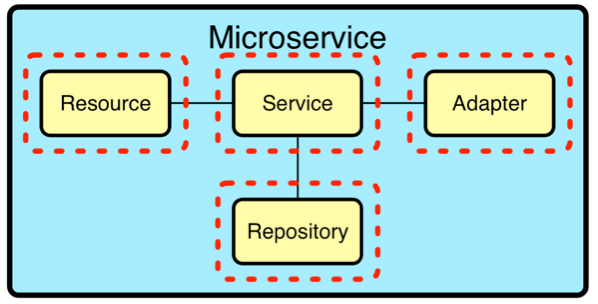
\includegraphics[ scale=0.37]{UnitTest}}
			\only<2>{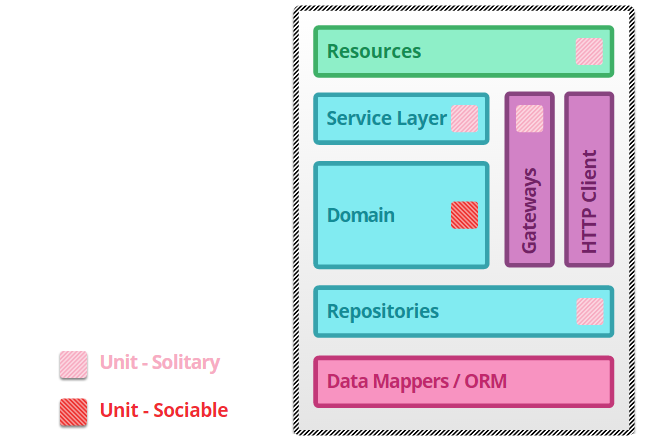
\includegraphics[ scale=0.34]{UnitTest2}}
			
 					\end{center} % image is from David Drake article and  -  Add Reference 
	\end{figure}
\end{column}
\end{columns}
\end{frame}


%===============================
% Intermediate Layer - To be revised
%===============================


\begin{frame}
	\frametitle{Types of Tests}	
	\framesubtitle{Integration,Component and Contract Testing }
Integration Tests
\begin{columns}
 \begin{column}{.49\textwidth}
	\begin{itemize}
		\item Covers communication paths and interactions between components to detect interface defects.
		\item Gateway Integration and Persistence Integration
		
	\end{itemize}
\end{column}
\begin{column}{.49\textwidth}
	\begin{figure}
		\begin{center}
 			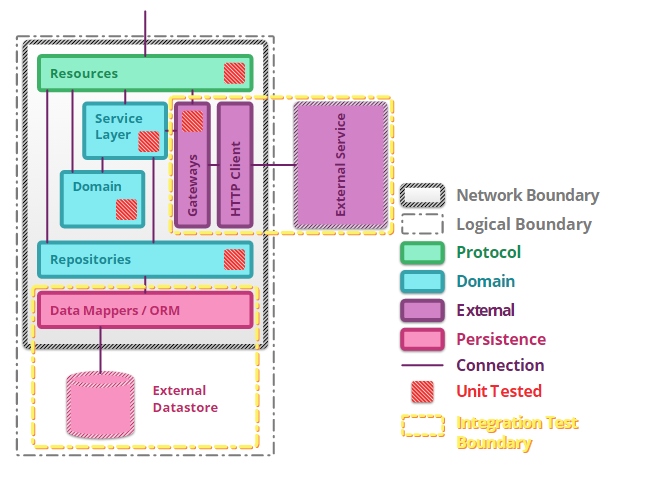
\includegraphics[ scale=0.37]{IntegrationTest}
 					\end{center} % image is from M.Fowler article -  Add Reference 
	\end{figure}
\end{column}
\end{columns}
\end{frame}


\begin{frame}
	\frametitle{Types of Tests}	
	\framesubtitle{Integration,Component and Contract Testing }
Integration Tests
\begin{columns}
 \begin{column}{.49\textwidth}
	\begin{itemize}
		\item A component is any well-encapsulated, coherent and independently replaceable part of a larger system.
		\item Isolation of the service is achieved by replacing external collaborators with test doubles
		
	\end{itemize}
\end{column}
\begin{column}{.49\textwidth}
	\begin{figure}
		\begin{center}
 			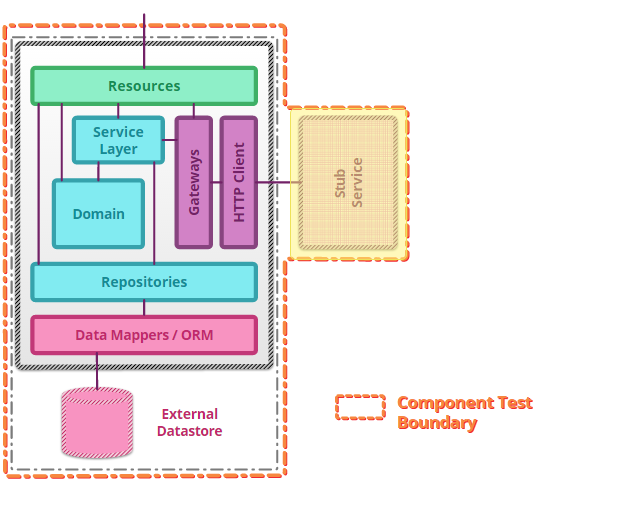
\includegraphics[ scale=0.3]{comptests}
 					\end{center} % image is from M.Fowler article -  Add Reference 
	\end{figure}
\end{column}
\end{columns}
\end{frame}


\begin{frame}
	\frametitle{Types of Tests}	
	\framesubtitle{Integration,Component and Contract Testing}
Contract Tests
\begin{columns}
 \begin{column}{.9\textwidth}
	\begin{itemize}
		\item Verifies that the contract expected by a consuming service is met.
		\item Integration Contract Testing and Consumer Driver Contract Testing.
\item The Overall Service contract is the sum of individual contract tests.
		
	\end{itemize}
\end{column}

\end{columns}
\end{frame}


\begin{frame}
\frametitle{Types of Tests}	
	\framesubtitle{Non Functional Tests}
Non Functional Tests validate the quality characteristics of the component.
\begin{columns}
 \begin{column}{.9\textwidth}
	\begin{itemize}
		\item Performance Tests.
		\item Tests for Scalability.
		\item Resiliency Tests.
		\item Security Tests.

		
	\end{itemize}
\end{column}

\end{columns}
\end{frame}


%===============================
%Test Scenarios
%===============================
\section{Test Scenarios}

\begin{frame}
	\frametitle{Testing between Microservices internal to an application or residing within the same application}
	\framesubtitle{ Interaction between the Aggregator and Data Loader.}
		\begin{center}
 			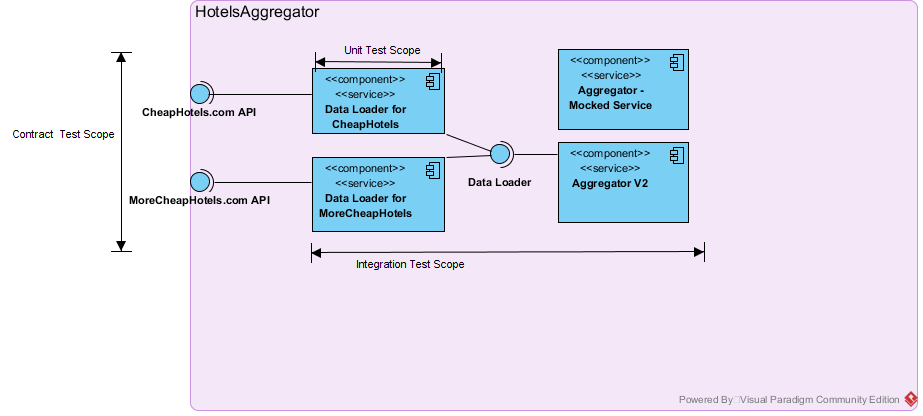
\includegraphics[ scale=0.4]{Scenario1}
 					\end{center} 

\end{frame}



\begin{frame}
	\frametitle{Testing between an internal microservice and an external API}
	\framesubtitle{Interaction with a Payment API}
		\begin{center}
 			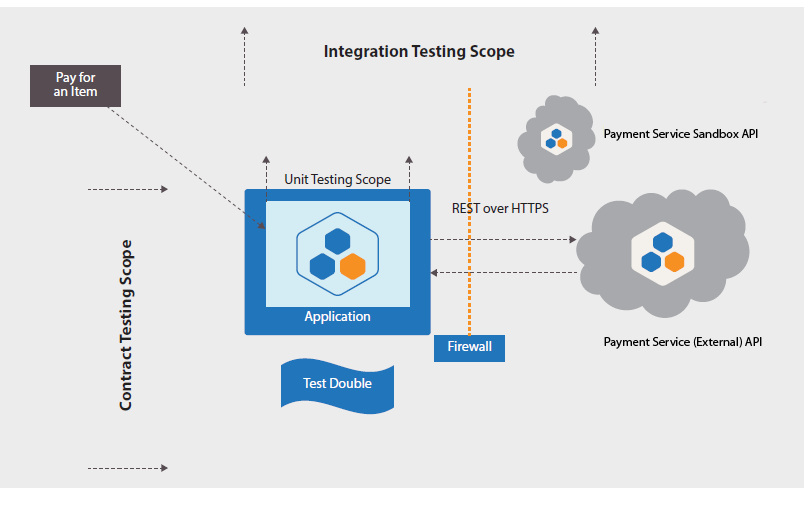
\includegraphics[ scale=0.5]{Scenario2}
 					\end{center} 
	
\end{frame}


\begin{frame}
	\frametitle{Microservice exposed to public domain}
	\framesubtitle{A publicly exposed application which is accessed by a Web API }
		\begin{center}
 			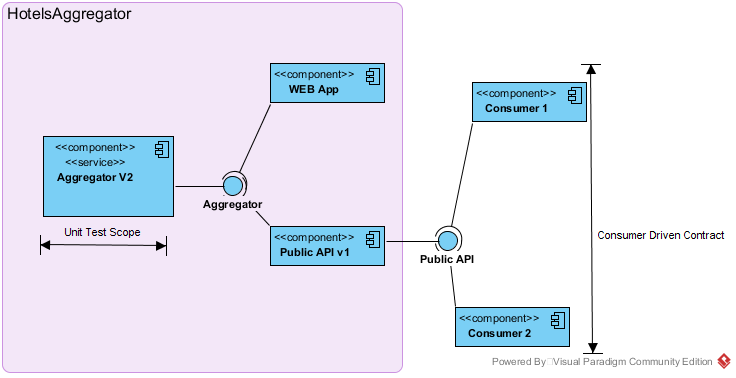
\includegraphics[ scale=0.5]{Scenario3}
 					\end{center} 
	
\end{frame}





%===============================
% CD related slides
%===============================
\section{Deployment}

\begin{frame}
	\frametitle{Deployment}
	\framesubtitle{Rapid Application Delivery}
	\begin{itemize}
		\item RAD is a prerequisite for microservices []
		\item Exhaustive tests could be slow.
		\item Remedy: Deployment Pipeline.
	\end{itemize}
\end{frame}

\begin{frame}
	\frametitle{Deployment}
	\framesubtitle{Deployment Pipeline}
	\begin{figure}
		\begin{center}
			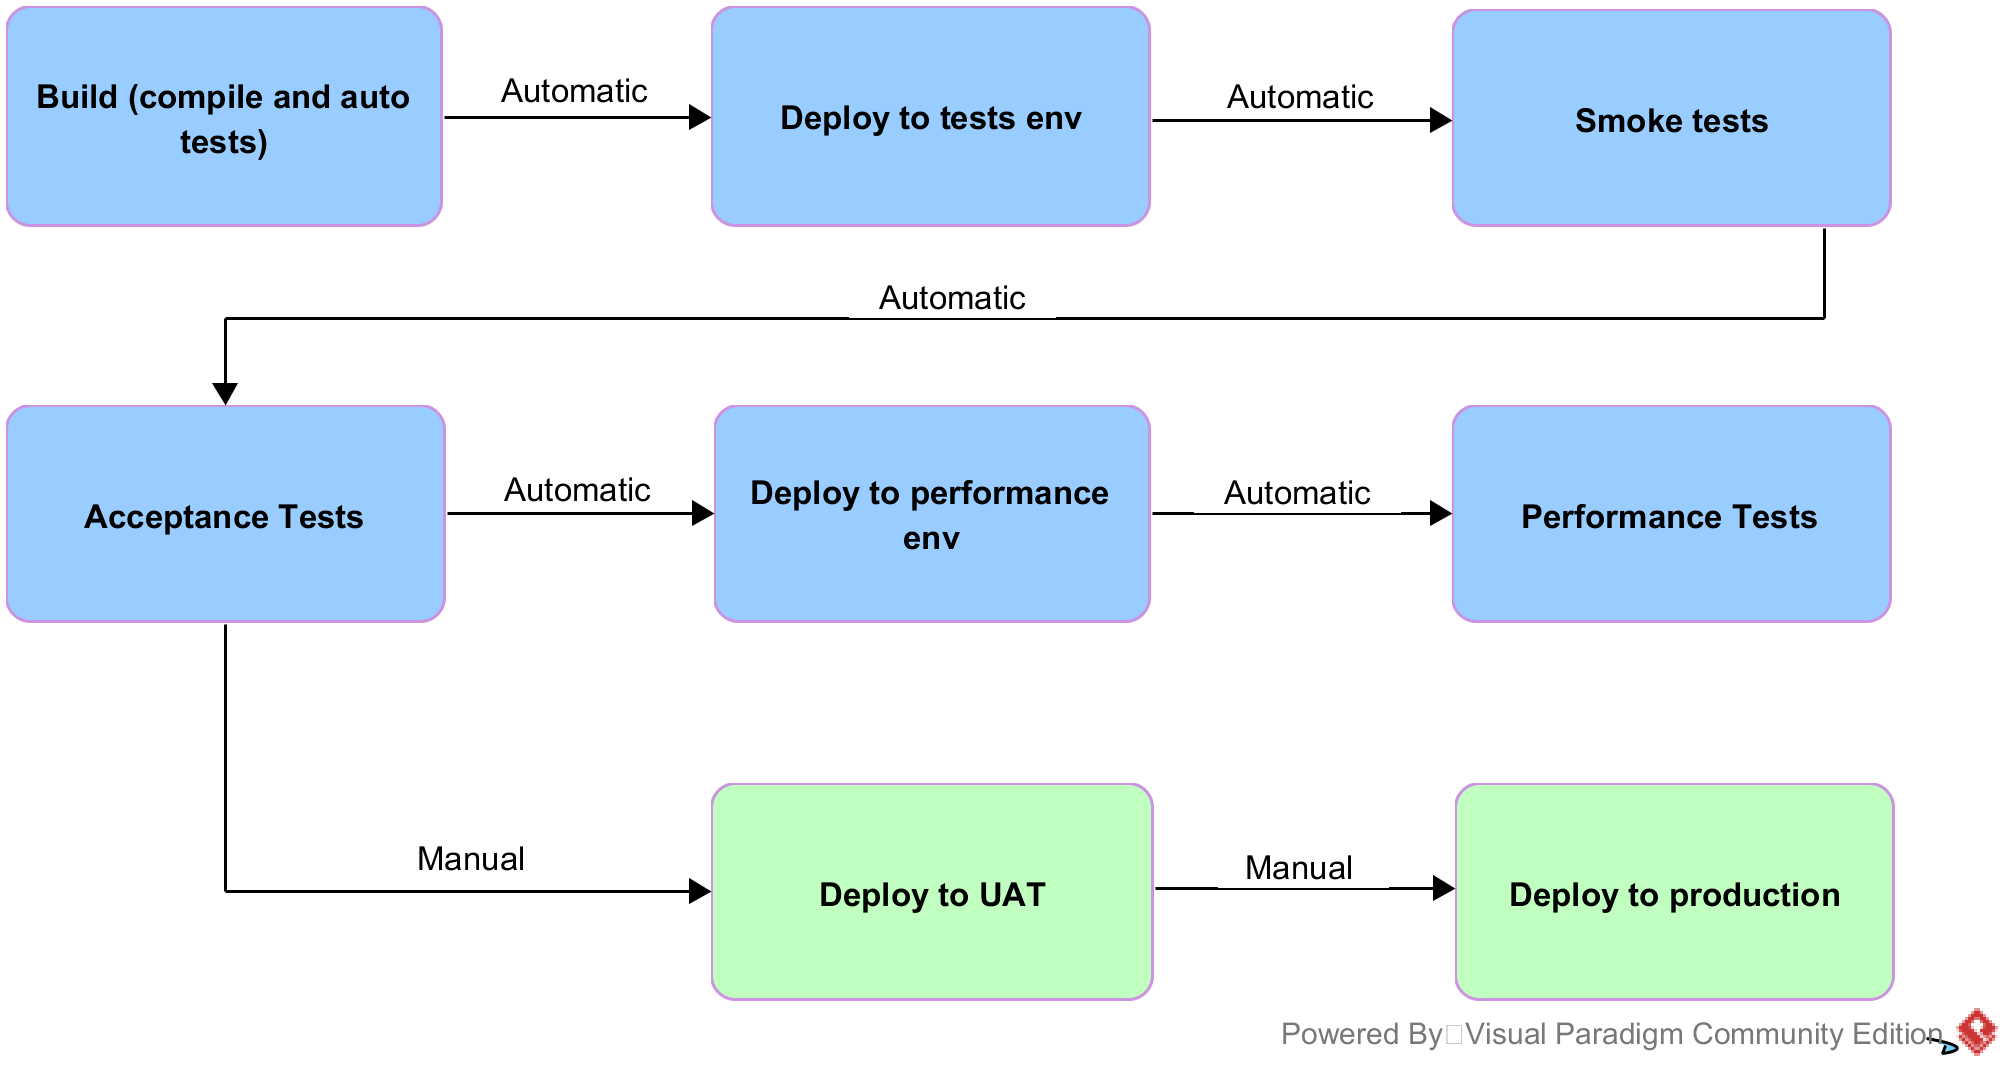
\includegraphics[ scale=0.6]{pipeline}
		\end{center}
	\end{figure}
\end{frame}

\begin{frame}
	\frametitle{Deployment}
	\framesubtitle{Continuous Deployment and Delivery}
	\begin{figure}
		\begin{center}
%https://puppet.com/blog/continuous-delivery-vs-continuous-deployment-what-s-diff
			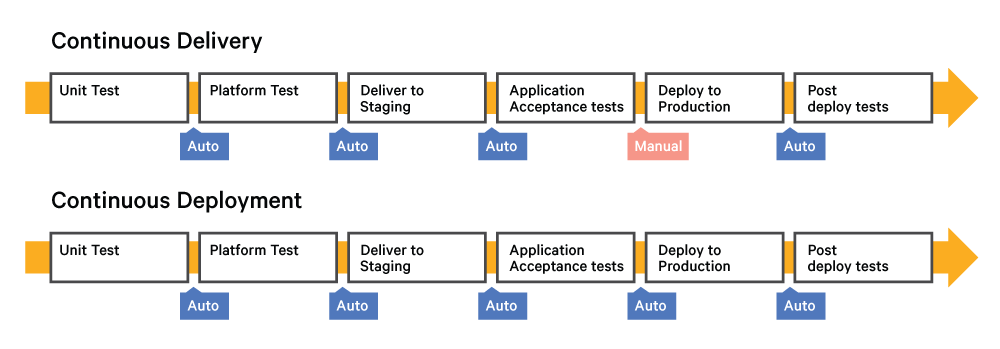
\includegraphics[scale=0.5]{delivery}
		\end{center}
	\end{figure}
\end{frame}

\begin{frame}
	\frametitle{Deployment}
	\framesubtitle{DevOps Culture}

DevOps Culture:
	\begin{itemize}
		\item Aim: break silos between development and later stages 
		\item Requirements: shared responsibility and autonomy of teams
	\end{itemize}
	\begin{figure}
		\begin{center}
% image is from http://blogs.atlassian.com/2016/03/how-to-choose-devops-tools/
% reference it!
 			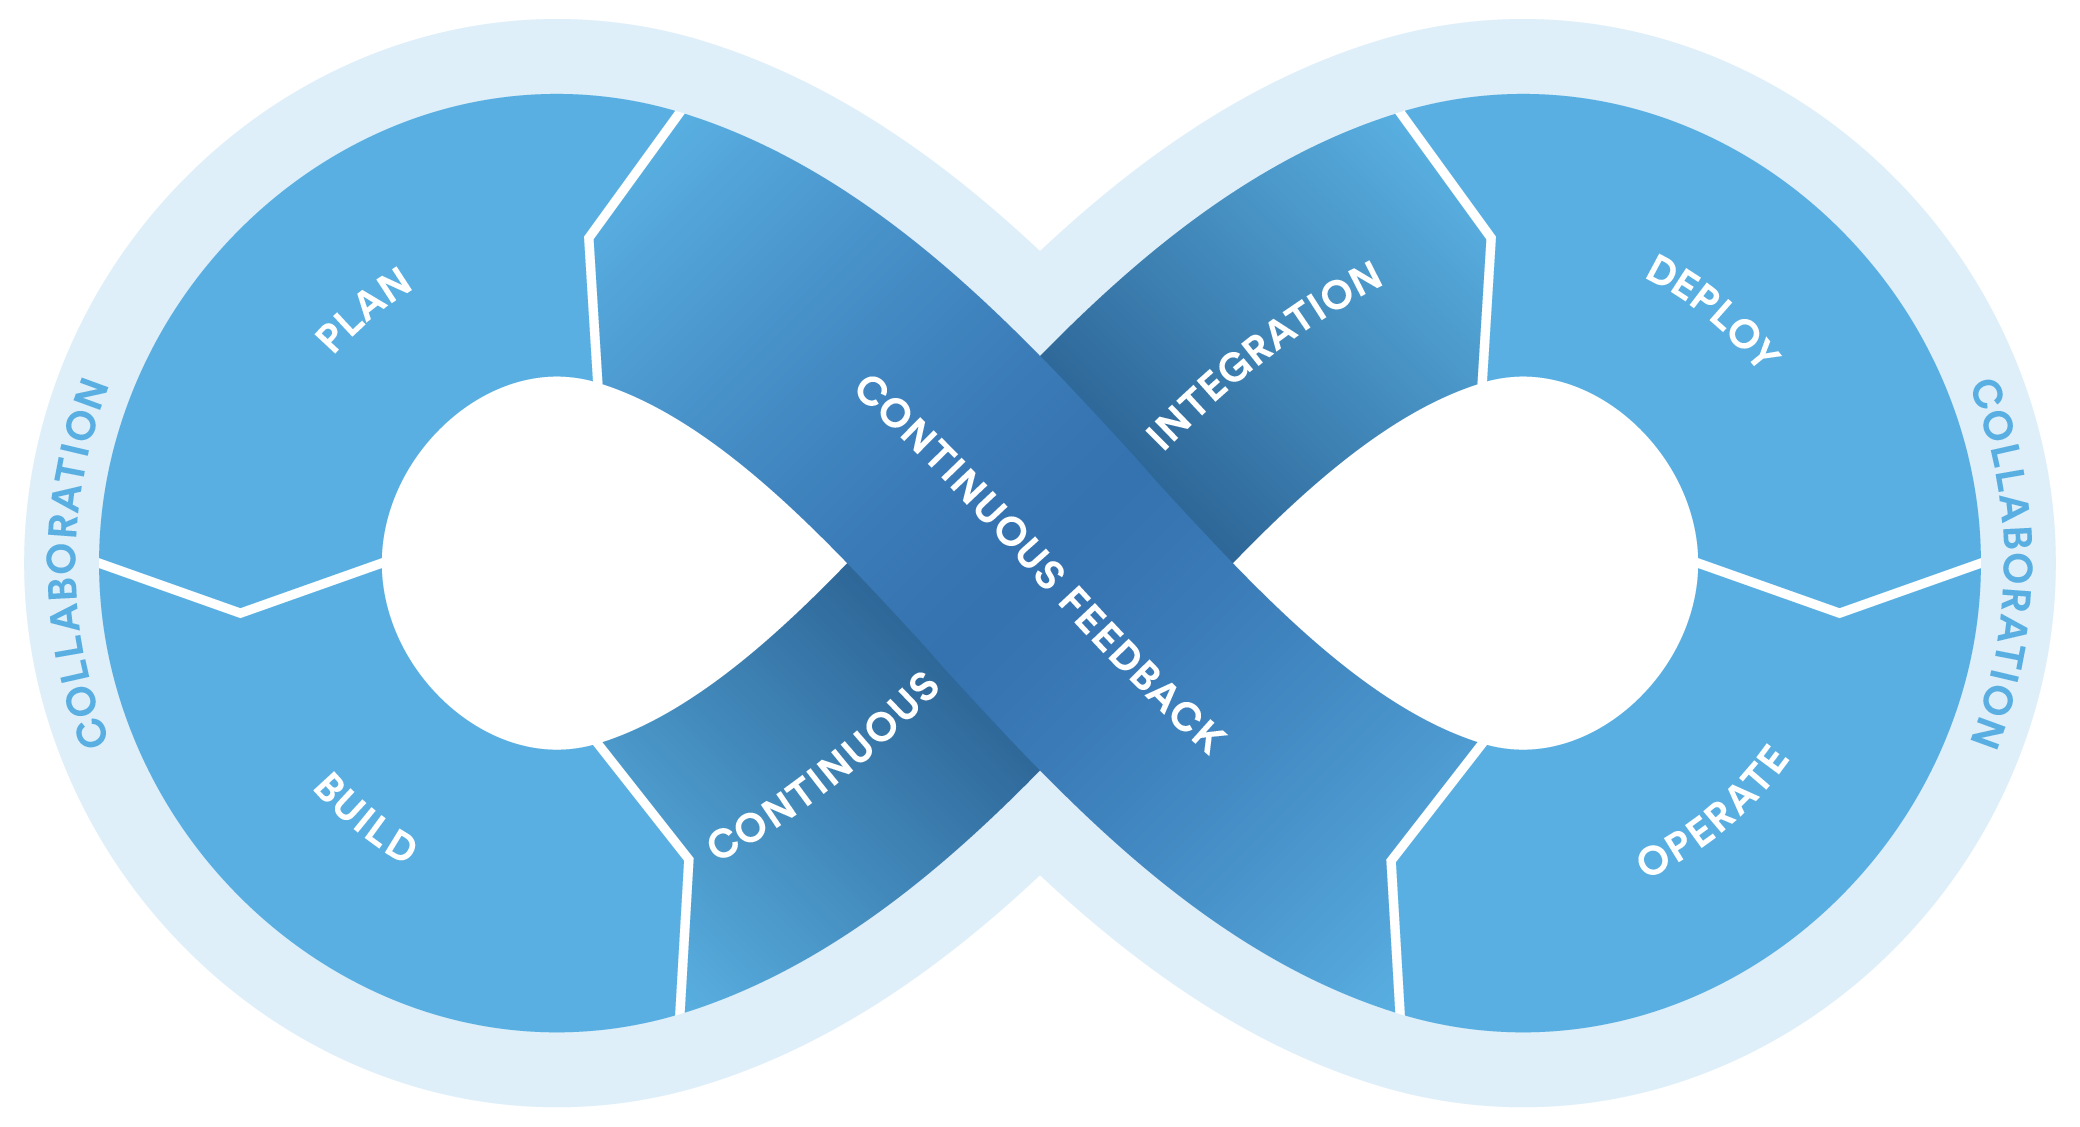
\includegraphics[scale=0.12]{devopsloop}
			\caption{\cite{devops}}
		\end{center}
	\end{figure}

\end{frame}


%===============================Start
% Smart releases slides
%===============================End
\section{After Deployment}

\begin{frame}
	\frametitle{After Deployment}
	\framesubtitle{Smart releasing strategies}
\begin{columns}
 \begin{column}{.49\textwidth}
	\begin{itemize}
		\item Smoke Test Suites
		\item Blue/Green Deployment
		\item Canary releasing
	\end{itemize}
\end{column}
\begin{column}{.49\textwidth}
	\begin{figure}
		\begin{center}
 			\only<1>{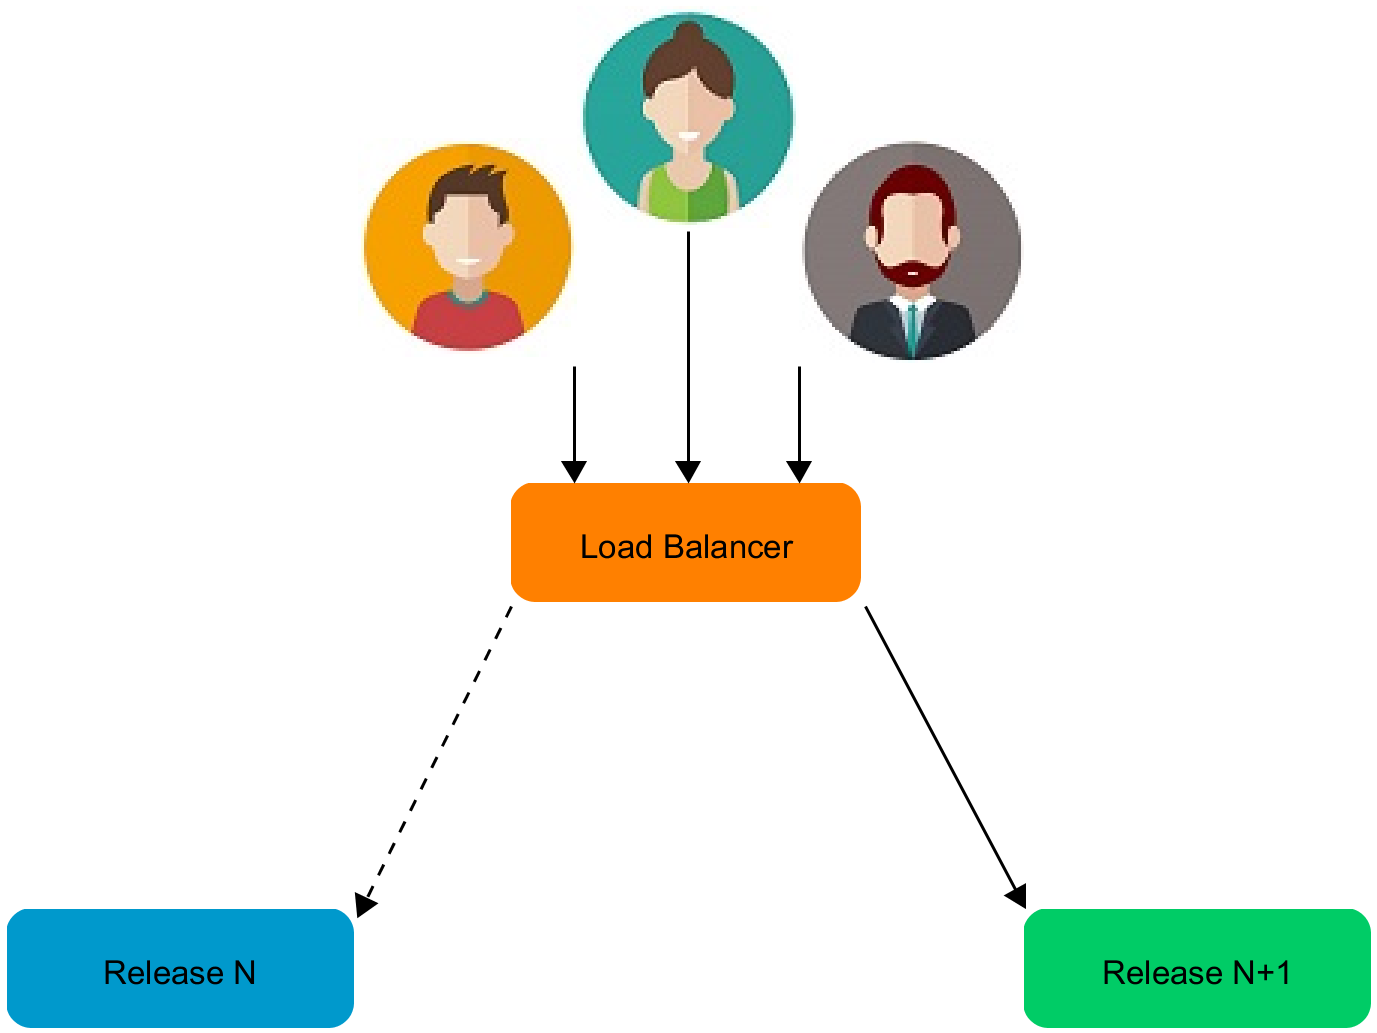
\includegraphics[ scale=0.5]{blue_green2}\\}
 			\only<2>{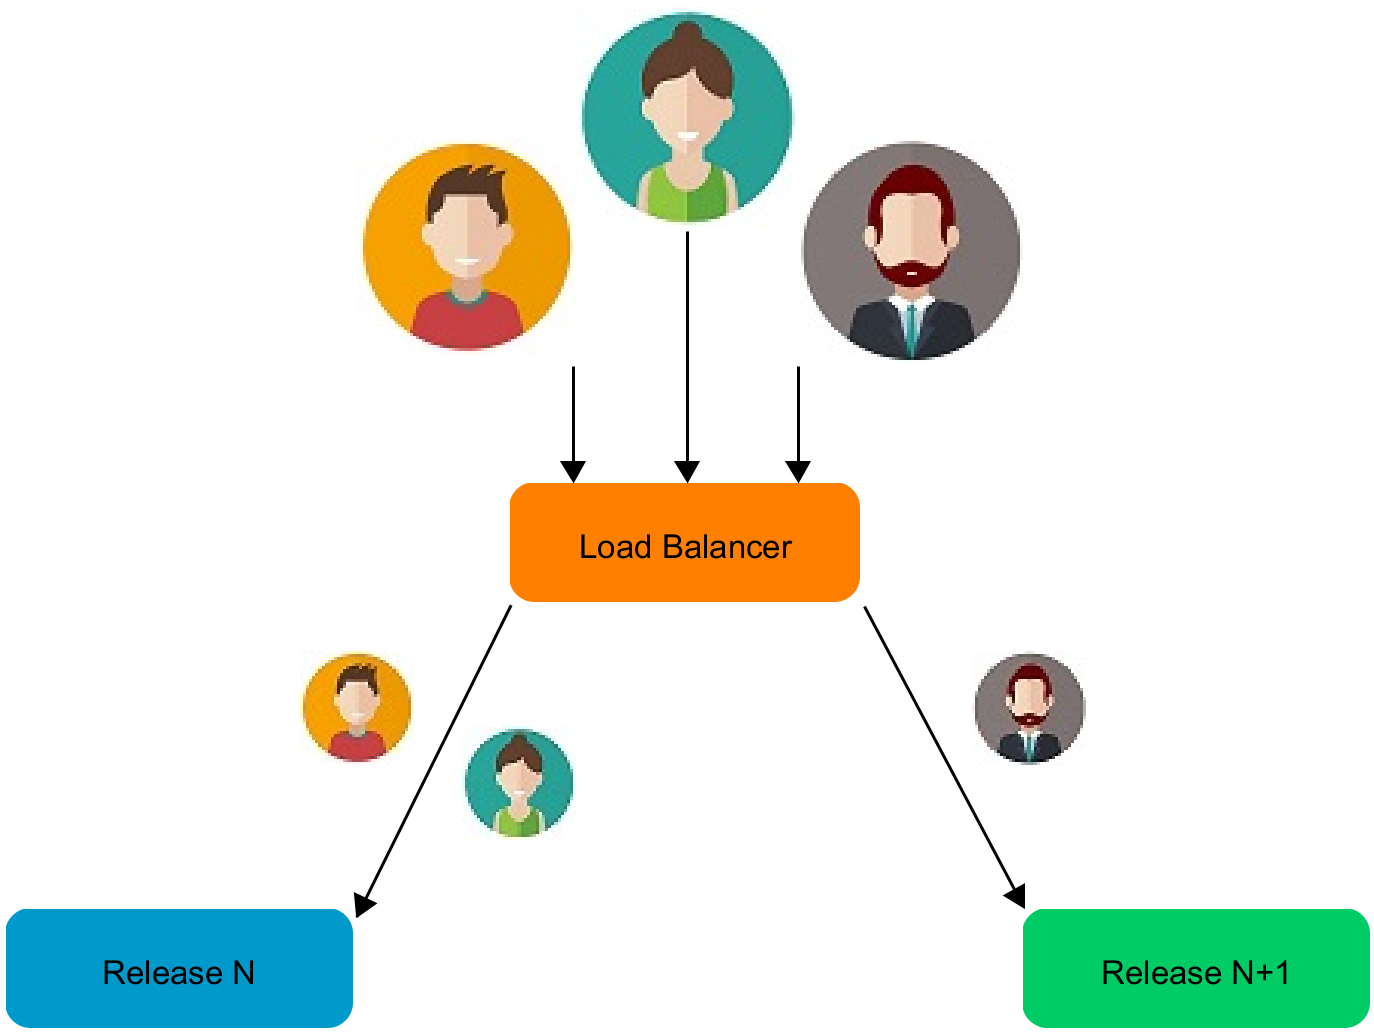
\includegraphics[ scale=0.5]{canary2}}\par
		\end{center}
	\end{figure}
\end{column}
\end{columns}
\end{frame}

\begin{frame}
	\frametitle{After Deployment}
	\framesubtitle{Logging}
In microservice architectures, log aggregator is required to see an application state.
\vfill
Example: use elastic stack to organize metrics.
	\begin{figure}
		\begin{center}
			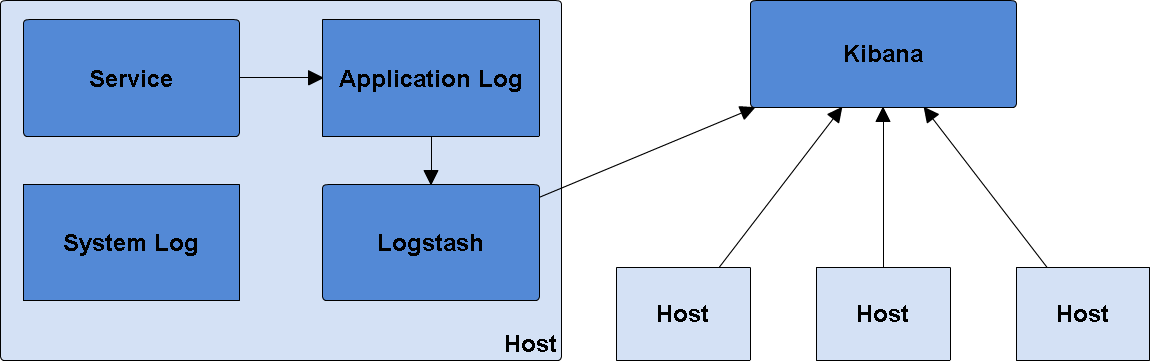
\includegraphics[scale=0.6]{logging}
		\end{center}
	\end{figure}
\end{frame}

\begin{frame}
	\frametitle{After Deployment}
	\framesubtitle{Monitoring}
\end{frame}

\begin{frame}
	\frametitle{Conclusion}
	\framesubtitle{}
	\begin{itemize}
		\item 
		\item 
	\end{itemize}
\end{frame}

%==============================Start
% References section
\section{References}
\begin{frame}
	\frametitle{References}
	\framesubtitle{}

	% make a list even without citation
        \nocite{newman,cohn,infosys,clemson,fowler_cont_del,naik}
	\bibliography{references}
\end{frame}

%===============================End


\end{document}
